\section{Problema k-PMP}

El problema k-PMP se reduce en encontrar todas las posibles k-Particiones del conjunto de v\'ertices de un grafo y de ellas, obtener las de menor suma total de aristas intrapartici\'on. Hallar las particiones de un conjunto ya fue resuelto previamente en otro trabajo pr\'actico de la c\'atedra y se puede relacionar con otros problemas de igual complejidad.

\subsection{k-PMP y el problema 3 del TP1}

El ejercicio 3 del TP1, consist\'ia en ubicar productos en camiones, teniendo en cuenta cierta peligrosidad entre cada par de productos y un umbral de peligrosidad propio de cada cami\'on. El objetivo era minimizar la cantidad de camiones, por lo que era necesario poner los productos de manera que las peligrosidades de a pares fueran m\'inimas y de esa forma, colocar la mayor cantidad de productos en cada cami\'on.

Para resolverlo se utiliz\'o la t\'ecnica de \textbf{Backtracking} y la idea b\'asicamente era que el primer producto se pod\'ia ubicar en el primer cam\'ion, el segundo, en el primer cami\'on o en su defecto crear uno nuevo, el tercero, en los camiones ya utilizados, (uno o dos) o colocar uno nuevo, etc. Se demostr\'o que para n productos, cada hoja del \'arbol de backtracking era una posible partici\'on de un conjunto de n elementos, pues nos podmeos abstraer de los productos y los camiones, y hablar de elementos y conjuntos, entonces el razonamiento se convierte en ubicar el primer elemento en un subconjunto nuevo, el segundo en el subconjunto que ya ten\'iamos o en un segundo conjunto, el tercero en los conjuntos ya utilizados o uno nuevo, etc. El \'arbol resultante ten\'ia la pinta de la \textbf{Figura \ref{combinaciones_4}}.

\begin{figure}[H]
	\begin{center}
		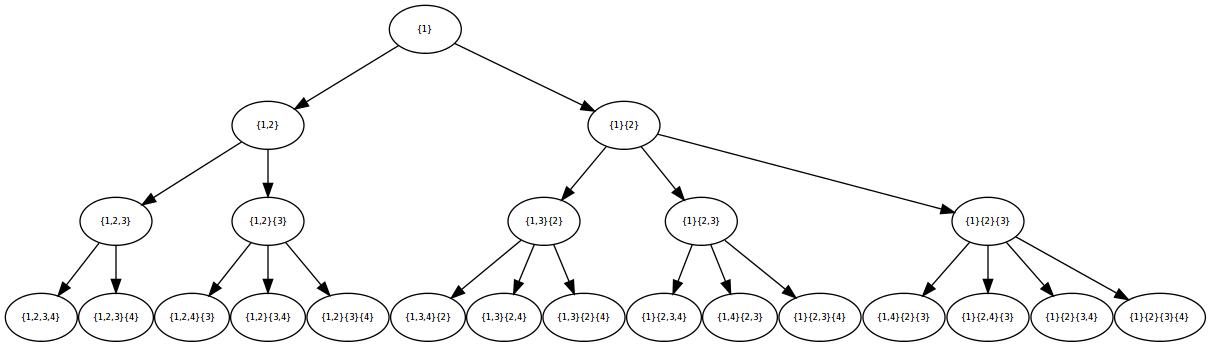
\includegraphics[scale=0.4]{ej1/combinaciones_4.jpg}
	\end{center}
	\caption{\'Arbol de combinaciones para tres elementos}
	\label{combinaciones_4}
\end{figure}

Si queremos hallar la mejor soluci\'on para el problema k-PNP debemos explorar todas las posibles k-Particiones y esto es un subconjunto de todas las particiones exploradas por el algoritmo de backtracking del Ejercicio 3 del TP1, por lo que s\'olo es necesario evitar las particiones que no nos interesan, es decir, aquellas con m\'as de k conjuntos o aquellas con menos, aunque esto \'ultimo es simplemente una decisi\'on de dise\~no explicada m\'as adelante.

\subsection{k-PMP y el problema de coloreo de v\'ertices de un grafo}

¿Qu\'e sucede si el peso de una k-PMP es cero? En tal caso tendr\'iamos una k-partici\'on tal que no existen aristas intrapartici\'on, es decir, obtenemos k conjuntos independientes de v\'ertices.

Si a cada conjunto se le asigna un color obtenemos un coloreo v\'alido para el grafo (esto sucede siempre y cuando el grafo sea ponderado con aristas de peso positivo mayor estricto que cero). Si el peso de la k-Partici\'on no es cero, existe alguna arista tal que dos v\'ertices del mismo conjunto son adyacentes, lo que imposibilita colorear. 

Por otro lado, sabemos que si la soluci\'on del problema k-PMP no es cero para un cierto k, tampoco lo va a ser para $k' < k$ pues si lo fuera, podr\'iamos partir de la soluci\'on de $k'-PMP$ y reducir el peso agreg\'andole un conjunto nuevo, sacando al menos un v\'ertice que tenga un adyacente el mismo conjuntos de los $k'$ calculados. 

Adem\'as si $k = |V|$ utilizando un conjunto para cada v\'ertice la suma ser\'ia cero. Por lo tanto un algoritmo para resolver coloreo ser\'ia resolver k-PMP para k=1, luego para k=2, as\'i hasta llegar a un k-PMP donde el peso sea cero. 

En cuanto a la complejidad, ser\'ia $n$ por la complejidad del algoritmo \'optimo de k-PMP.

Es sabido que encontrar el m\'inimo $k$ para colorear un grafo es un problema NP-Completo, por lo que se reafirma el hecho de que k-PMP tambi\'en lo es, porque si no lo fuera, coloreo se podr\'ia resolver con el algoritmo antes mencionado y no ser\'ia NP-C.

\subsection{k-PMP y modelado de problemas reales}

Este modelo matem\'atico puede ser aplicado a diferentes situaciones
en donde se disponen de recursos y se busca la mejor manera de que
trabajen juntos.

Por ejemplo en la computación distribuida, cada vértice puede ser una
computadora y cada arista la velocidad de la conexión entre un par de
ellas.

Si el problema admite ser dividido en K subproblemas independientes
entre si, 
entonces se puede buscar K conjuntos de computadoras para que trabajen
en simultaneo y ataquen cada uno de estos K subproblemas minimizando
la pérdida producida por la red.
Como los mismos son independientes las computadoras de las distintas
particiones no necesitan comunicarse entre si hasta terminar el
problema y las comunicaciones intra partición son óptimas.

Para el caso anterior habría que restringuir la no existencia de
aristas para evitar computadoras no conectadas en alguna partición.

Otro grupo de problemas para los cuales sirve son los de cableado,
donde es deseable eliminar las conexiones de mayor costo. Un ejemplo
de esto es VLSI (Very Large Scale Integration).

También tienen relación con tareas de secuenciamiento de trabajos, de
una forma similar al ejemplo de computo en paralelo, lo que se puede
buscar mediante un modelado en grafo y un algoritmo que resuelva
k-PMP es que tareas o trabajos no conviene hacer en simultaneo.
Cada partición tendría entonces las tareas que pueden correr en
simultaneo con un menor costo global.